\documentclass{../homework}

\title{Homework 1}
% \author{Tim Randolph}
\date{COMS W3261, Summer A 2022}

\begin{document}

\maketitle

This homework is due \textbf{Tuesday, 5/31/2022, at 11:59pm EST}. Submit to GradeScope (course code: 2KGDW8).

\textbf{Grading policy reminder:} \LaTeX~is preferred, but neatly typed or handwritten solutions are acceptable.\footnote{The website \href{https://www.overleaf.com/}{Overleaf} (essentially Google Docs for LaTeX) may make compiling and organizing your .tex files easier. Here's a quick \href{https://www.overleaf.com/learn/latex/Learn_LaTeX_in_30_minutes}{tutorial}.} I recommend using the .tex file for the homework as a template to write up your answers. Your TAs may dock points for indecipherable writing.\\

Proofs should be complete; that is, include enough information that a reader can clearly tell that the argument is rigorous. \\

If a question is ambiguous, please state your assumptions. This way, we can give you credit for correct work. (Even better, post on Ed so that we can resolve the ambiguity.) \\

\textbf{\LaTeX~resources.}
\begin{itemize}
    \item \href{https://detexify.kirelabs.org/classify.html}{Detexify} is a nice tool that lets you draw a symbol and returns the \LaTeX~codes for similar symbols. 
    \item The tool \href{https://www.tablesgenerator.com/}{Table Generator} makes building tables in \LaTeX~much easier.
    \item The tool \href{http://madebyevan.com/fsm/}{Finite State Machine Designer} may be useful for drawing automata. See also this example (\href{https://static.us.edusercontent.com/files/HZeTXimODzWeLvHIqsvjL2BG}{PDF}) (\href{https://static.us.edusercontent.com/files/RI3W8tQNvHMWFe9MkXV1KztA}{.tex}) of how to make making fancy edges (courtesy of Eumin Hong).
    \item The website \href{https://www.mathcha.io/}{mathcha.io} allows you to draw diagrams and convert them to \LaTeX~code.
    \item To use the previous drawing tools (and for most drawing in \LaTeX), you'll need to use the package Tikz (add the command ``\textbackslash usepackage\{tikz\}'' to the preamble of your .tex file to import the package). 
    \item \href{https://www.overleaf.com/learn/latex/Positioning_of_Figures}{This tutorial} is a helpful guide to positioning figures.
\end{itemize}  

\clearpage

\section{Problem 1 (6 points)}

    % Note: the following Tikz code was generated using http://madebyevan.com/fsm/
    \begin{center}
    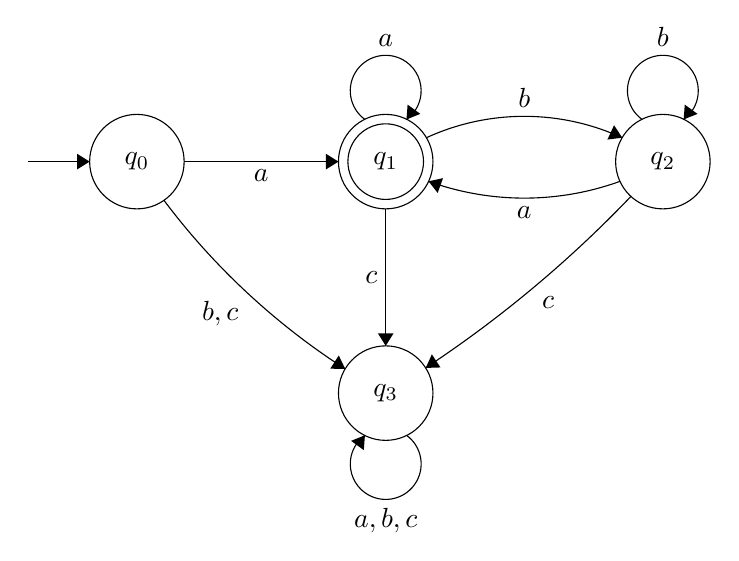
\begin{tikzpicture}[scale=0.2]
    \tikzstyle{every node}+=[inner sep=0pt]
    \draw [black] (22.4,-21.9) circle (3);
    \draw (22.4,-21.9) node {$q_0$};
    \draw [black] (38.2,-21.9) circle (3);
    \draw (38.2,-21.9) node {$q_1$};
    \draw [black] (38.2,-21.9) circle (2.4);
    \draw [black] (55.8,-21.9) circle (3);
    \draw (55.8,-21.9) node {$q_2$};
    \draw [black] (38.2,-36.6) circle (3);
    \draw (38.2,-36.6) node {$q_3$};
    \draw [black] (25.4,-21.9) -- (35.2,-21.9);
    \fill [black] (35.2,-21.9) -- (34.4,-21.4) -- (34.4,-22.4);
    \draw (30.3,-22.4) node [below] {$a$};
    \draw [black] (35.625,-35.062) arc (-122.78154:-143.08744:44.574);
    \fill [black] (35.63,-35.06) -- (35.22,-34.21) -- (34.68,-35.05);
    \draw (27.69,-30.71) node [below] {$b,c$};
    \draw [black] (38.2,-24.9) -- (38.2,-33.6);
    \fill [black] (38.2,-33.6) -- (38.7,-32.8) -- (37.7,-32.8);
    \draw (37.7,-29.25) node [left] {$c$};
    \draw [black] (36.877,-19.22) arc (234:-54:2.25);
    \draw (38.2,-14.65) node [above] {$a$};
    \fill [black] (39.52,-19.22) -- (40.4,-18.87) -- (39.59,-18.28);
    \draw [black] (40.782,-20.383) arc (114.66769:65.33231:14.898);
    \fill [black] (53.22,-20.38) -- (52.7,-19.59) -- (52.28,-20.5);
    \draw (47,-18.52) node [above] {$b$};
    \draw [black] (53.078,-23.152) arc (-70.11635:-109.88365:17.869);
    \fill [black] (40.92,-23.15) -- (41.5,-23.89) -- (41.84,-22.95);
    \draw (47,-24.72) node [below] {$a$};
    \draw [black] (53.771,-24.109) arc (-43.70207:-56.55883:75.848);
    \fill [black] (40.74,-35) -- (41.68,-34.97) -- (41.13,-34.14);
    \draw (48.51,-30.41) node [below] {$c$};
    \draw [black] (39.523,-39.28) arc (54:-234:2.25);
    \draw (38.2,-43.85) node [below] {$a,b,c$};
    \fill [black] (36.88,-39.28) -- (36,-39.63) -- (36.81,-40.22);
    \draw [black] (15.5,-21.9) -- (19.4,-21.9);
    \fill [black] (19.4,-21.9) -- (18.6,-21.4) -- (18.6,-22.4);
    \draw [black] (54.477,-19.22) arc (234:-54:2.25);
    \draw (55.8,-14.65) node [above] {$b$};
    \fill [black] (57.12,-19.22) -- (58,-18.87) -- (57.19,-18.28);
    \end{tikzpicture}
    \end{center}

\begin{enumerate}
    \item (3 points.) The DFA state diagram above is defined on the alphabet $\Sigma = \{a,b,c\}$. Write out its formal definition (as a 5-tuple). When specifying the transition function $\delta$, you can draw a table or simply describe the output of $\delta$ on all possible inputs. 
    
    \item (3 points.) Describe the language recognized by the DFA in one sentence, then explain why the DFA accepts a string if and only if it matches your description. [Hint: Test some strings and look for a pattern; never forget the empty string $\epsilon$!]
    
    \end{enumerate}
    
\blfootnote{ Rationale: The goal of this question is to make sure you're comfortable reading state diagrams, evaluating DFAs on strings, and reasoning about what they do. }
\blfootnote{ References: Sipser 1.1 pp. 34-37; Lightning review of DFAs linked in the Lecture 1 \href{https://docs.google.com/document/d/1PHCNkMitYsMpbh-sxrBmr-cGbpUEshfdFDS2k09fHrI}{Course Skeleton}.}
    
\clearpage
\section{Problem 2 (8 points).}
    \begin{enumerate}
    \item (4 points.) Consider the DFA drawn below. What is the language recognized by this DFA (over what alphabet)? Describe your reasoning.
    
    \begin{center}
    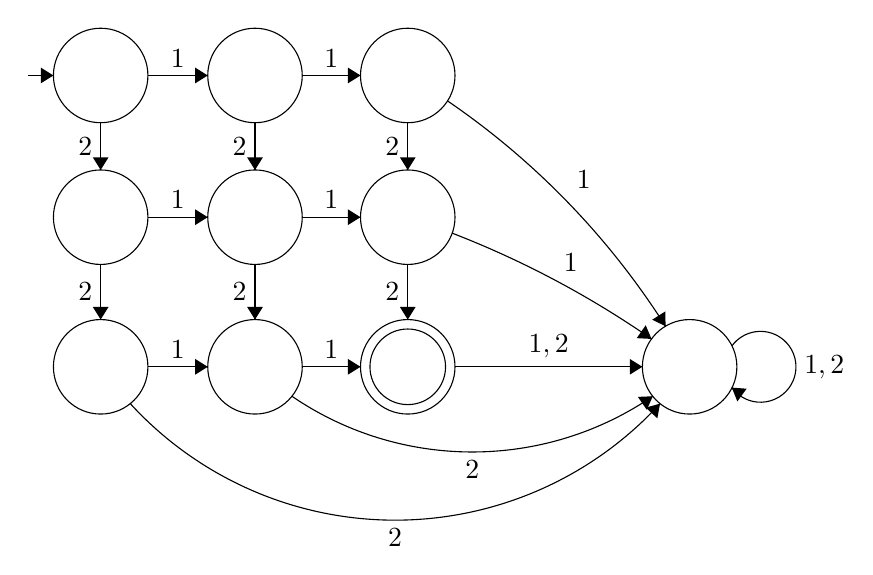
\begin{tikzpicture}[scale=0.2]
    \tikzstyle{every node}+=[inner sep=0pt]
    \draw [black] (16.5,-11.5) circle (3);
    \draw [black] (26.3,-11.5) circle (3);
    \draw [black] (36,-11.5) circle (3);
    \draw [black] (16.5,-20.5) circle (3);
    \draw [black] (26.3,-20.5) circle (3);
    \draw [black] (36,-20.5) circle (3);
    \draw [black] (16.5,-30) circle (3);
    \draw [black] (26.3,-30) circle (3);
    \draw [black] (36,-30) circle (3);
    \draw [black] (36,-30) circle (2.4);
    \draw [black] (53.9,-30) circle (3);
    \draw [black] (11.9,-11.5) -- (13.5,-11.5);
    \fill [black] (13.5,-11.5) -- (12.7,-11) -- (12.7,-12);
    \draw [black] (19.5,-11.5) -- (23.3,-11.5);
    \fill [black] (23.3,-11.5) -- (22.5,-11) -- (22.5,-12);
    \draw (21.4,-11) node [above] {$1$};
    \draw [black] (29.3,-11.5) -- (33,-11.5);
    \fill [black] (33,-11.5) -- (32.2,-11) -- (32.2,-12);
    \draw (31.15,-11) node [above] {$1$};
    \draw [black] (16.5,-14.5) -- (16.5,-17.5);
    \fill [black] (16.5,-17.5) -- (17,-16.7) -- (16,-16.7);
    \draw (16,-16) node [left] {$2$};
    \draw [black] (16.5,-23.5) -- (16.5,-27);
    \fill [black] (16.5,-27) -- (17,-26.2) -- (16,-26.2);
    \draw (16,-25.25) node [left] {$2$};
    \draw [black] (26.3,-14.5) -- (26.3,-17.5);
    \fill [black] (26.3,-17.5) -- (26.8,-16.7) -- (25.8,-16.7);
    \draw (25.8,-16) node [left] {$2$};
    \draw [black] (26.3,-23.5) -- (26.3,-27);
    \fill [black] (26.3,-27) -- (26.8,-26.2) -- (25.8,-26.2);
    \draw (25.8,-25.25) node [left] {$2$};
    \draw [black] (36,-14.5) -- (36,-17.5);
    \fill [black] (36,-17.5) -- (36.5,-16.7) -- (35.5,-16.7);
    \draw (35.5,-16) node [left] {$2$};
    \draw [black] (36,-23.5) -- (36,-27);
    \fill [black] (36,-27) -- (36.5,-26.2) -- (35.5,-26.2);
    \draw (35.5,-25.25) node [left] {$2$};
    \draw [black] (19.5,-20.5) -- (23.3,-20.5);
    \fill [black] (23.3,-20.5) -- (22.5,-20) -- (22.5,-21);
    \draw (21.4,-20) node [above] {$1$};
    \draw [black] (29.3,-20.5) -- (33,-20.5);
    \fill [black] (33,-20.5) -- (32.2,-20) -- (32.2,-21);
    \draw (31.15,-20) node [above] {$1$};
    \draw [black] (19.5,-30) -- (23.3,-30);
    \fill [black] (23.3,-30) -- (22.5,-29.5) -- (22.5,-30.5);
    \draw (21.4,-29.5) node [above] {$1$};
    \draw [black] (29.3,-30) -- (33,-30);
    \fill [black] (33,-30) -- (32.2,-29.5) -- (32.2,-30.5);
    \draw (31.15,-29.5) node [above] {$1$};
    \draw [black] (38.527,-13.116) arc (55.67361:32.43769:49.421);
    \fill [black] (52.37,-27.42) -- (52.36,-26.48) -- (51.52,-27.01);
    \draw (46.7,-18.09) node [right] {$1$};
    \draw [black] (38.823,-21.513) arc (68.84403:55.24383:60.5);
    \fill [black] (51.48,-28.23) -- (51.11,-27.36) -- (50.54,-28.18);
    \draw (46.35,-23.99) node [above] {$1$};
    \draw [black] (39,-30) -- (50.9,-30);
    \fill [black] (50.9,-30) -- (50.1,-29.5) -- (50.1,-30.5);
    \draw (44.95,-29.5) node [above] {$1,2$};
    \draw [black] (52.024,-32.338) arc (-42.51426:-137.48574:22.824);
    \fill [black] (52.02,-32.34) -- (51.11,-32.59) -- (51.85,-33.27);
    \draw (35.2,-40.24) node [below] {$2$};
    \draw [black] (51.557,-31.869) arc (-55.65859:-124.34141:20.309);
    \fill [black] (51.56,-31.87) -- (50.61,-31.91) -- (51.18,-32.73);
    \draw (40.1,-35.91) node [below] {$2$};
    \draw [black] (56.58,-28.677) arc (144:-144:2.25);
    \draw (61.15,-30) node [right] {$1,2$};
    \fill [black] (56.58,-31.32) -- (56.93,-32.2) -- (57.52,-31.39);
    \end{tikzpicture}
    \end{center}
    
    \item (4 points.) Draw a state diagram for a DFA \textbf{with at most 4 states} that recognizes the language over the alphabet $\Sigma = \{1, 2, 3\}$ consisting of all strings of digits that never decrease (that is, we never see a $1$ after we've seen a $2$ or a $3$, or a $2$ after we've seen a $3$.)
    
    Explain in words why your DFA recognizes the language specified.
 
\end{enumerate}

\blfootnote{ Rationale: More practice reading state diagrams and evaluating DFAs on strings; also, practice designing DFAs to perform a task and simplifying them. }
\blfootnote{ References: Sipser 1.1 pp. 34-37 (DFAs); Sipser 1.1 pp. 41-43 (designing DFAs); Lightning reviews of DFAs and designing DFAs linked in the Lecture 1 \href{https://docs.google.com/document/d/1PHCNkMitYsMpbh-sxrBmr-cGbpUEshfdFDS2k09fHrI}{Course Skeleton}.}



\clearpage
\section{Problem 3 (8 points)}

\begin{enumerate}
    \item (3 points). Draw a state diagram for an NFA on the alphabet $\Sigma = \{0\}$ that recognizes the language
    \[
        L = \{w \; | \; |w| \text{ is divisible by 3 or by 5 (or by both 3 and 5). } \}.
    \]
    (Recall that $|w|$ denotes the length of the string $w$.) Explain in words why your NFA recognizes the language specified.
    
    
    \item (5 points). Draw the state diagram of a DFA (with alphabet $\Sigma = \{0,1\}$) \textbf{with at most 3 states} that recognizes the same language as the NFA whose state diagram is pictured below. Explain in words why your DFA captures the same language as the original NFA. [Hint: A DFA with three states can only do so much. So, if this question is possible, the NFA below must be simpler than it seems. Try to work out what it does (testing strings is never a bad option.)]
    
    \begin{center}
    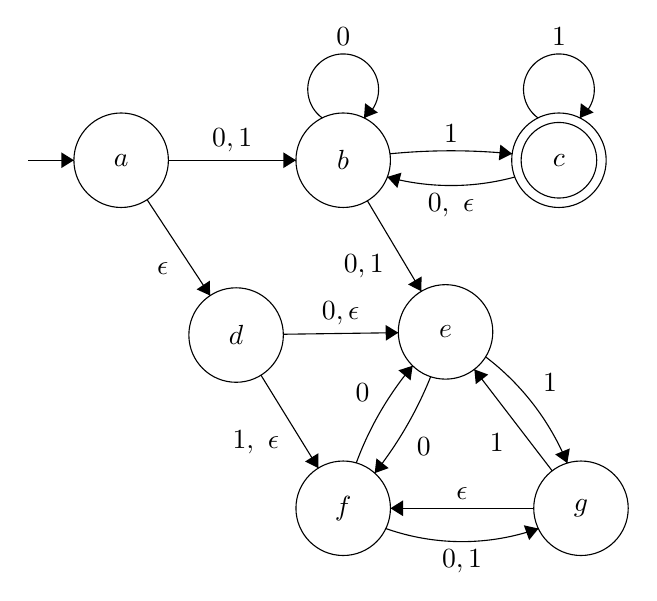
\begin{tikzpicture}[scale=0.2]
    \tikzstyle{every node}+=[inner sep=0pt]
    \draw [black] (16.8,-17.7) circle (3);
    \draw (16.8,-17.7) node {$a$};
    \draw [black] (30.9,-17.7) circle (3);
    \draw (30.9,-17.7) node {$b$};
    \draw [black] (44.6,-17.7) circle (3);
    \draw (44.6,-17.7) node {$c$};
    \draw [black] (44.6,-17.7) circle (2.4);
    \draw [black] (24.1,-28.8) circle (3);
    \draw (24.1,-28.8) node {$d$};
    \draw [black] (37.4,-28.6) circle (3);
    \draw (37.4,-28.6) node {$e$};
    \draw [black] (30.9,-39.8) circle (3);
    \draw (30.9,-39.8) node {$f$};
    \draw [black] (46,-39.8) circle (3);
    \draw (46,-39.8) node {$g$};
    \draw [black] (10.9,-17.7) -- (13.8,-17.7);
    \fill [black] (13.8,-17.7) -- (13,-17.2) -- (13,-18.2);
    \draw [black] (19.8,-17.7) -- (27.9,-17.7);
    \fill [black] (27.9,-17.7) -- (27.1,-17.2) -- (27.1,-18.2);
    \draw (23.85,-17.2) node [above] {$0,1$};
    \draw [black] (29.577,-15.02) arc (234:-54:2.25);
    \draw (30.9,-10.45) node [above] {$0$};
    \fill [black] (32.22,-15.02) -- (33.1,-14.67) -- (32.29,-14.08);
    \draw [black] (33.871,-17.291) arc (95.65197:84.34803:39.384);
    \fill [black] (41.63,-17.29) -- (40.88,-16.71) -- (40.78,-17.71);
    \draw (37.75,-16.6) node [above] {$1$};
    \draw [black] (43.277,-15.02) arc (234:-54:2.25);
    \draw (44.6,-10.45) node [above] {$1$};
    \fill [black] (45.92,-15.02) -- (46.8,-14.67) -- (45.99,-14.08);
    \draw [black] (41.8,-18.765) arc (-74.75802:-105.24198:15.407);
    \fill [black] (33.7,-18.76) -- (34.34,-19.46) -- (34.6,-18.49);
    \draw (37.75,-19.81) node [below] {$0,\mbox{ }\epsilon$};
    \draw [black] (18.45,-20.21) -- (22.45,-26.29);
    \fill [black] (22.45,-26.29) -- (22.43,-25.35) -- (21.59,-25.9);
    \draw (19.84,-24.58) node [left] {$\epsilon$};
    \draw [black] (32.44,-20.28) -- (35.86,-26.02);
    \fill [black] (35.86,-26.02) -- (35.88,-25.08) -- (35.02,-25.59);
    \draw (33.51,-24.41) node [left] {$0,1$};
    \draw [black] (27.1,-28.75) -- (34.4,-28.65);
    \fill [black] (34.4,-28.65) -- (33.59,-28.16) -- (33.61,-29.16);
    \draw (30.74,-28.18) node [above] {$0,\epsilon$};
    \draw [black] (25.68,-31.35) -- (29.32,-37.25);
    \fill [black] (29.32,-37.25) -- (29.33,-36.3) -- (28.48,-36.83);
    \draw (26.87,-35.58) node [left] {$1,\mbox{ }\epsilon$};
    \draw [black] (31.731,-36.92) arc (159.76269:139.97923:20.763);
    \fill [black] (35.31,-30.75) -- (34.41,-31.04) -- (35.18,-31.68);
    \draw (32.6,-32.44) node [left] {$0$};
    \draw [black] (36.455,-31.445) arc (-21.85898:-38.39911:24.608);
    \fill [black] (32.9,-37.57) -- (33.79,-37.25) -- (33.01,-36.63);
    \draw (35.55,-35.87) node [right] {$0$};
    \draw [black] (43.296,-41.086) arc (-70.4877:-109.5123:14.507);
    \fill [black] (43.3,-41.09) -- (42.37,-40.88) -- (42.71,-41.82);
    \draw (38.45,-42.42) node [below] {$0,1$};
    \draw [black] (43,-39.8) -- (33.9,-39.8);
    \fill [black] (33.9,-39.8) -- (34.7,-40.3) -- (34.7,-39.3);
    \draw (38.45,-39.3) node [above] {$\epsilon$};
    \draw [black] (39.943,-30.184) arc (52.77355:22.26468:16.175);
    \fill [black] (45.13,-36.93) -- (45.29,-36) -- (44.36,-36.38);
    \draw (43.56,-31.8) node [right] {$1$};
    \draw [black] (44.17,-37.42) -- (39.23,-30.98);
    \fill [black] (39.23,-30.98) -- (39.32,-31.92) -- (40.11,-31.31);
    \draw (41.13,-35.61) node [left] {$1$};
    \end{tikzpicture}
    \end{center}

    
\end{enumerate}

\blfootnote{Rationale: The purpose of this question is to get experience in building, testing, and simplifying NFAs. }
\blfootnote{References: Sipser 1.2 pp. 47-53 (NFAs), also see the Lightning Review video on NFAs linked in the \href{https://docs.google.com/document/d/1PHCNkMitYsMpbh-sxrBmr-cGbpUEshfdFDS2k09fHrI}{Course Skeleton}. }

\clearpage
\section{Problem 4 (8 points)}

\begin{enumerate}
    \item (5 points.) Given languages $A$ and $B$, define the $XNOR$ operation $\odot$ as follows:
    \[
        A \odot B := \{x \; | \; x \in (A \cap B), \text{ or } x \in (\overline{A} \cap \overline{B})\}.
    \]
    Prove that the class of regular languages is closed under $\odot$ by showing that, given two arbitrary DFAs $D_1$ and $D_2$, we can build a new DFA $D_3$ that recognizes the language $L(D_1) \odot L(D_2)$. [Hint: recall our proof that the regular languages are closed under the union operation, available on p.45 of Sipser.]
    
    
    \item (3 points.) Prove that the class of regular languages is closed under $\odot$ in a different way: by reasoning from the fact that the regular languages are closed under union, intersection, Kleene star, and complement (you may assume these facts without proof.)
\end{enumerate}

\blfootnote{Rationale: The goal of this question is to get comfortable building DFAs programmatically (combining two generic DFAs using their formal definitions), and also thinking about the logic of closure (if $X$ and $Y$ are regular and the regular languages are closed under $\clubsuit$, then $X \clubsuit Y$ is regular).}
\blfootnote{References: Sipser pp.45-46 (proof that the regular languages are closed under the union operation), \href{https://en.wikipedia.org/wiki/Closure_(mathematics)}{Wiki: Closure}.}

\clearpage
\section{Problem 5 (9 points)}

\begin{enumerate}
    \item (9 points). Consider the language $L$ on the alphabet $\{0, 1, 2\}$ consisting of all strings that meet both of the following conditions:
    \begin{itemize}
        \item Every 0 is immediately followed by a 1, every 1 is immediately followed by a 2, and every 2 is immediately followed by an 0.
        \item The string starts and ends with the same digit.
    \end{itemize}
    For example, the strings `1', `0120120', and `1201' are in the language, while `111', `210', and `012012' are not.
    \begin{enumerate}
        \item (6 points). Show that the following languages are regular:
        \begin{enumerate}
            \item $L_{inc}$, the language of strings over $\{0,1,2\}$ such that every 0 is immediately followed by a 1, every 1 is immediately followed by a 2, and every 2 is immediately followed by an 0.
            
            \item $L_0$, $L_1$, and $L_2$, the languages of strings over $\{0, 1, 2\}$ that start and end in 0, 1, and 2 respectively.
            
        \end{enumerate}
        \item (3 points). Use closure properties of the regular languages (closure under union, intersection, concatenation, etc), along with your results from the previous part to conclude that $L$ is regular.
        
    \end{enumerate}
\end{enumerate}

\blfootnote{Rationale: The point of this question is to practice combining several types of regularity proofs including using DFAs, NFAs, and closure properties. }
\blfootnote{References: Sipser 1.2 pp. 47-53 (NFAs), the Lightning Review video on NFAs linked in the \href{https://docs.google.com/document/d/1PHCNkMitYsMpbh-sxrBmr-cGbpUEshfdFDS2k09fHrI}{Course Skeleton}, \href{https://en.wikipedia.org/wiki/Closure_(mathematics)}{Wiki: Closure}. }


\clearpage
\section{Problem 6 (1 point)}
    \begin{enumerate}
        \item What was the muddiest (most confusing) point of class during week 1, in your opinion?
        
        \item What was your favorite part of class during week 1?
        
        \item (Optional) Any other thoughts? Thank you!
    \end{enumerate}

\blfootnote{Rationale: We'll spend more time reviewing the toughest topics from each week, and we'll repeat the activities that are most useful. }

\end{document}
